
\documentclass[tcc]{ppgccufmg} % utilizem 'tcc' para a monografia final ou 'proposal' para projeto de TCC

% configura��es do documento
\usepackage[brazil]{babel}      % se o documento for em portugu�s
\usepackage[latin1]{inputenc}
%\usepackage[utf8]{inputenc}	% devo usar esse pacote ?  (!)
\usepackage[T1]{fontenc} 
\usepackage{graphicx}
\usepackage[a4paper,
portuguese,
bookmarks=true,
bookmarksnumbered=true,
linktocpage,
colorlinks,
citecolor=black,
urlcolor=blue,
linkcolor=blue,
filecolor=black,
]{hyperref}
\usepackage[square]{natbib}


\begin{document}
	
	% O comando a seguir, \ppgccufmg, prov� todas as informa��es relevantes para a
	% classe ppgccufmg. Por favor, consulte a documenta��o para a descri��o de
	% cada chave.
	
	% Um exemplo para documentos em portugu�s � apresentado a seguir:
	\ppgccufmg{
		title={Job-Shop Scheduling\\com abordagem Just-in-Time},
		authorrev={Rodrigues Jardim, Filipi Maciel},
		cutter={D1234p},   % dados que futuramente ser�o utilizados pela biblioteca
		cdu={519.6*82.10}, % dados que futuramente ser�o utilizados pela biblioteca (!)
		university={Instituto Federal do Norte de Minas Gerais},
		campus={Montes Claros},
		coursetype = {Bacharelado},
		course={Ci�ncia da Computa��o},
		address={Montes Claros},
		date={2024-03},
		keywords={Job-Shop, Scheduling, Just-in-Time, JSSP},
		advisor={Tadeu Zubaran}, % nome completo de tadeu? (!)
		%  approval={img/approvalsheet.eps},  (!)
		abstract={Resumo}{resumo},
		abstract=[english]{Abstract}{abstract},
		dedication={dedicatoria}, % n�o consegui encontrar o arquivo/vari�vel para alterar (!)
		ack={agradecimentos},
		epigraphtext={It's not darkness that deceives and hides. It's light.}{Death Note},
	}
	
	% LISTA DE EPIGRAFES 
	% It's not darkness that deceives and hides. It's light - Death Note
	% O que � melhor? Nascer bom ou superar sua natureza maligna com muito esfor�o? - Paarthurnax, The Elder Scrolls 5: Skyrim
	% The right man in the wrong place can make all the difference in the world. - G-Man, Half-Life 2
	% Stand in the ashes of a trillion dead souls, and asks the ghosts if honor matters. The silence is your answer. -  Javik, Mass Effect 3
	% The harder you beat a man, the taller he stands. - The Jackal, Far Cry 2
	% 
	
	
	% caso tenha a necessidade de incluir algumas configura��es adicionais...
	% Os três comandos seguintes são apenas para gerar texto para ocupar espaço nas
% páginas.
\newcommand{\dummytxta}{%
Lorem ipsum dolor sit amet, consectetur adipisicing elit, sed do
eiusmod tempor incididunt ut labore et dolore magna aliqua. Ut enim ad
minim veniam, quis nostrud exercitation ullamco laboris nisi ut
aliquip ex ea commodo consequat. Duis aute irure dolor in
reprehenderit in voluptate velit esse cillum dolore eu fugiat nulla
pariatur. Excepteur sint occaecat cupidatat non proident, sunt in
culpa qui officia deserunt mollit anim id est laborum.\par
}

\newcommand{\dummytxtb}{%
Sed ut perspiciatis unde omnis iste natus error sit voluptatem accusantium
doloremque laudantium, totam rem aperiam, eaque ipsa quae ab illo inventore
veritatis et quasi architecto beatae vitae dicta sunt explicabo. Nemo enim
ipsam voluptatem quia voluptas sit aspernatur aut odit aut fugit, sed quia
consequuntur magni dolores eos qui ratione voluptatem sequi nesciunt. Neque
porro quisquam est, qui dolorem ipsum quia dolor sit amet, consectetur,
adipisci velit, sed quia non numquam eius modi tempora incidunt ut labore et
dolore magnam aliquam quaerat voluptatem. Ut enim ad minima veniam, quis
nostrum exercitationem ullam corporis suscipit laboriosam, nisi ut aliquid ex
ea commodi consequatur? Quis autem vel eum iure reprehenderit qui in ea
voluptate velit esse quam nihil molestiae consequatur, vel illum qui dolorem
eum fugiat quo voluptas nulla pariatur?\par
}

\newcommand{\dummytxtc}{%
At vero eos et accusamus et iusto odio dignissimos ducimus qui blanditiis
praesentium voluptatum deleniti atque corrupti quos dolores et quas molestias
excepturi sint occaecati cupiditate non provident, similique sunt in culpa qui
officia deserunt mollitia animi, id est laborum et dolorum fuga. Et harum
quidem rerum facilis est et expedita distinctio. Nam libero tempore, cum soluta
nobis est eligendi optio cumque nihil impedit quo minus id quod maxime placeat
facere possimus, omnis voluptas assumenda est, omnis dolor
repellendus. Temporibus autem quibusdam et aut officiis debitis aut rerum
necessitatibus saepe eveniet ut et voluptates repudiandae sint et molestiae non
recusandae. Itaque earum rerum hic tenetur a sapiente delectus, ut aut
reiciendis voluptatibus maiores alias consequatur aut perferendis doloribus
asperiores repellat.\par
}

\newcommand{\dummytxt}{\dummytxta\dummytxtb\dummytxtc}
	
	% Inclua cada cap�tulo em um arquivo separado para melhorar a organiza��o
	\chapter{Introdu��o}

Segundo \cite{horn86robot}, todo tri�ngulo equil�tero tem os lados iguais. J�
segundo \cite{shashua97photometric}, todo quadrado tamb�m tem.

Veja que o pacote \verb|natbib| permite uma s�rie de formas diferentes para
fazer refer�ncias bibliogr�ficas. O comando padr�o, \verb|\cite|, realiza a
cita��o comum vista no par�grafo anterior. Outros comandos permitem, por
exemplo, citar somente o autor --- por exemplo, citar o trabalho de
\citeauthor{samaras99coupled} --- ou colocar automaticamente a cita��o entre
par�nteses \citep{hougen93estimation, sato99illumination2, sato99illumination1,
sato01stability}. Os comandos usados foram, respectivamente, \verb|\citeauthor|
e \verb|\citep|. Veja a documenta��o do \verb|natbib| na Internet para conhecer
outros comandos e exemplos de uso. 

Cita��es aleat�rias para fazer com que as refer�ncias bibliogr�ficas ocupem
mais de uma p�gina: \cite{bichsel92simple, dror01statistics, guisser92new}.


\section{Motiva��o}

\dummytxtb\dummytxta

\subsection{Sub-motiva��o}


\dummytxtc\dummytxtb

\subsection{Mais uma sub-se��o}

\dummytxta\dummytxtc

\subsubsection{Descendo mais um n�vel}

\dummytxtb\dummytxta

	% \input{TrabalhosRelacionados}
	\chapter{Desenvolvimento}

\dummytxtb\dummytxta\dummytxtc

\begin{figure}[ht]
    \centering
    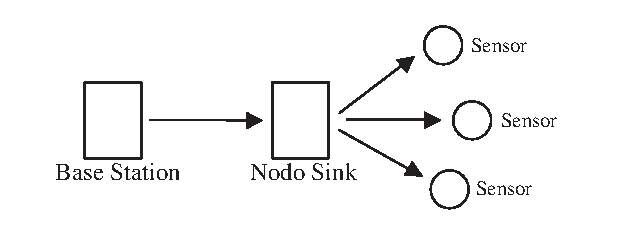
\includegraphics{img/exemplo}
    %\includegraphics[scale=.5]{exemplo-x}
    \caption{Uma figura de exemplo.}
\end{figure}

\dummytxtb

\begin{table}[ht]
    \caption{Uma tabela de exemplo.}
    {\centering
    \begin{tabular}{lcr} \toprule
    \emph{Left-aligned} & \emph{Centered} & \emph{Right-aligned} \\ \midrule
    Lorem ipsum & dolor sit & amet \\
    consectetur adipisicing & elit, sed do eiusmod & tempor \\
    incididunt ut & labore et dolore & magna aliqua. \\ \bottomrule
    \end{tabular}\par
    }
\end{table}

	% \input{Resultados}
	% \input{Conclusoes}
	
	% Aqui vem a parte da bibliografia: use o comando \ppgccbibliography indicando
	% apenas o nome do arquivo .bib (sem a extens�o).
	\ppgccbibliography{bibfile}
	
	
	% Este comando encapsula o conjunto de ap�ndices. A sua fun��o � fazer com que
	% a numera��o dos ap�ndices seja feita com letras mai�sculas (A, B, C, etc.) e
	% a palavra "Ap�ndice" anteceda as entradas no Sum�rio.
	\begin{appendices}
		% Para cada ap�ndice, um \chapter
\chapter{Um ap�ndice}

\dummytxta
\dummytxtb
\dummytxtc
\dummytxta
\dummytxtb
		\chapter{Outro ap�ndice}

\dummytxta
\dummytxtb
\dummytxtc
\dummytxta
\dummytxtb
	\end{appendices} % Fim dos ap�ndices (usar apenas depois do �ltimo ap�ndice)
	
	
	% Este comando encapsula o conjunto de anexos. A sua fun��o � fazer com que a
	% numera��o dos anexos seja feita com letras mai�sculas (A, B, C, etc.) e a
	% palavra "Anexo" anteceda as entradas no Sum�rio.
	\begin{attachments}
		% Para cada anexo, um \chapter
\chapter{Um anexo}

\dummytxta
\dummytxtb
\dummytxtc
\dummytxta
\dummytxtb
		\chapter{Outro anexo}

\dummytxta
\dummytxtb
\dummytxtc
\dummytxta
\dummytxtb
	\end{attachments} % Fim dos anexos (usar apenas depois do �ltimo anexo)
	
	
\end{document}
